\documentclass[tikz]{standalone}
\usepackage{pgfplots}
\pgfplotsset{compat=1.15}
\usepackage{mathrsfs}
\usetikzlibrary{arrows,calc}
\usepackage{tkz-euclide}
\pagestyle{empty}

\usepackage[greek,english]{babel}
\usepackage{textgreek}

\definecolor{AngleClr}{rgb}{0,0.39215686274509803,0}
\definecolor{ShapeClr}{rgb}{0.6,0.2,0}

\begin{document}

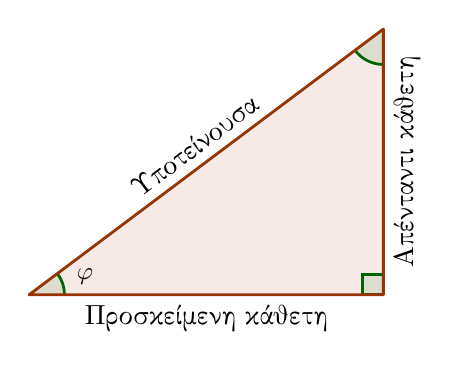
\begin{tikzpicture}[scale=.75]
\tkzSetUpLine[line width=1pt,color=black]
\tkzSetUpPoint[fill=black]

\tkzDefPoints{6/0/A,6/4.5/B,0/0/C}

\tkzFillPolygon[fill=ShapeClr,fill opacity=0.1](A,B,C)
\tkzMarkRightAngle[line width=1pt, size=.35,color=AngleClr,fill=AngleClr,fill opacity=0.1](B,A,C)
\tkzFillAngles[fill=AngleClr,size=.6,fill opacity=0.1](C,B,A A,C,B)
\tkzMarkAngles[line width=1pt,size=.6,color=AngleClr](C,B,A A,C,B)

\tkzDrawPolygon[color=ShapeClr](A,B,C)

\tkzLabelSegment[sloped,below](A,B){\textgreek{Απένταντι κάθετη}}
\tkzLabelSegment(A,C){\textgreek{Προσκείμενη κάθετη}}
\tkzLabelSegment[sloped, above](B,C){\textgreek{Υποτείνουσα}}

\tkzLabelAngle[pos=1](A,C,B){\scalebox{0.9}{$\varphi$}}

\end{tikzpicture}
\end{document}
